\section{Results}\label{sec:results}
\subsection{Simulator validation}\label{sec:valid}
Before any test run we checked the stick--slip emulation (protocol checks V1--V6, Table~\ref{tab:valid}). Slow-ramp breakaway occurred within 0.3--2.7\% of the nominal grip, for both $r=1$ and $r=1.2$. The contact itself has a small static/kinetic gap: breakaway at 0.988 and sliding at 0.980 of nominal capacity, an intrinsic ratio of 1.008, so an emulated $r=1.2$ measured 1.206. Creep in the stuck phase was below $10^{-5}$\,rad/s. Halving the time step changed first-slip travel by less than 0.025\,rad, and scaling both switching thresholds by 0.5 or 2 changed it by less than 0.01\,rad.

The direct test of Proposition~\ref{prop:pivot} held the rod at 1.01 times its measured breakaway grip and then released it to $q F_{\rm last}$ (Fig.~\ref{fig:bound}). Over 128 releases, simulated travel averaged 0.90--0.97 of the bound, so the bound is tight. However, 24 releases exceeded it, by at most 0.048\,rad, more than our 0.02\,rad sensing margin. We recorded this before testing (deviation D2) and expected certificate violations in the test runs.

\begin{table}[t]\centering\footnotesize
\caption{Simulator validation (validation objects only; recorded before any test data).}\label{tab:valid}
\begin{tabular}{@{}lll@{}}\toprule
Check & Quantity & Result\\\midrule
V1 & slow-ramp breakaway / nominal & 1.003--1.027\\
V2 & intrinsic static/kinetic ratio & 1.008 (1.006--1.010)\\
V2 & emulated $r=1.2$, measured & 1.206\\
V3 & creep at 1.05\,$F_h$ & $<10^{-5}$\,rad/s\\
V4 & first-slip travel, $dt$ halved & $|\Delta|<0.025$\,rad\\
V5 & thresholds $\times0.5$, $\times2$ & $|\Delta|<0.01$\,rad\\
V6 & travel / Prop.~1 bound & 0.90--0.97 (mean)\\
V6 & releases over bound & 24/128, max 0.048\,rad\\\bottomrule
\end{tabular}
\end{table}

\begin{figure}[t]\centering
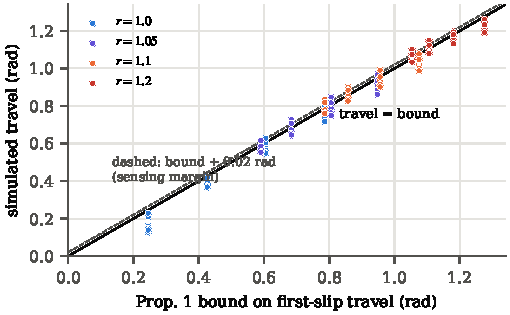
\includegraphics[width=\columnwidth]{fig_bound.pdf}
\caption{Proposition~\ref{prop:pivot} against simulation (V6). Each point is one release from a measured stuck grip. Points above the solid line exceed the bound; points above the dashed line exceed it by more than the sensing margin.}\label{fig:bound}
\end{figure}

\begin{table*}[t]\centering\footnotesize
\caption{Sliding test set (40 objects; learned methods: 5 seeds, 200 episodes per cell). Within: final error $\le$5\,mm and held. Over: travel past the target by more than 5\,mm. Probes: position measurements per episode. Shield $r_{\max}=1.2$.}\label{tab:slide}
\setlength{\tabcolsep}{3.2pt}
\begin{tabular}{llrrrrrrrrrrrr}
\toprule
 & & \multicolumn{3}{c}{$r=1.0$} & \multicolumn{3}{c}{$r=1.1$} & \multicolumn{3}{c}{$r=1.2$} & \multicolumn{3}{c}{$r=1.3$}\\
\cmidrule(lr){3-5}\cmidrule(lr){6-8}\cmidrule(lr){9-11}\cmidrule(lr){12-14}
ID & method & within & over & probes & within & over & probes & within & over & probes & within & over & probes\\
\midrule
B0 & model & 82 & 15 & 14.7 & 90 & 8 & 13.5 & 70 & 30 & 11.4 & 72 & 28 & 11.5\\
B0S & model + shield & 78 & \textbf{0} & 24.2 & 65 & 2 & 26.6 & 75 & 2 & 21.0 & 68 & 5 & 21.1\\
\midrule
B2 & residual & 90 & 8 & 9.3 & 90 & 10 & 8.2 & 89 & 11 & 7.4 & 86 & 13 & 7.9\\
B4 & residual, shield at test & 94 & 2 & 13.9 & 90 & 2 & 14.5 & 92 & \textbf{0} & 15.0 & 94 & \textbf{1} & 13.1\\
B5 & shield-trained residual & 98 & 2 & 12.1 & 98 & \textbf{1} & 11.9 & 96 & 2 & 11.4 & 96 & 2 & 10.8\\
\bottomrule
\end{tabular}
\end{table*}

\begin{table*}[t]\centering\footnotesize
\caption{Pivoting test set (40 objects; learned methods: 5 seeds, 200 episodes per cell). Within: final error $\le$0.05\,rad and held. Over: overshoot past the target by more than 0.05\,rad. Probes: angle measurements per pivot. Shield $r_{\max}=1.1$.}\label{tab:pivot}
\setlength{\tabcolsep}{3.2pt}
\begin{tabular}{llrrrrrrrrrrrr}
\toprule
 & & \multicolumn{3}{c}{$r=1.0$} & \multicolumn{3}{c}{$r=1.05$} & \multicolumn{3}{c}{$r=1.1$} & \multicolumn{3}{c}{$r=1.2$}\\
\cmidrule(lr){3-5}\cmidrule(lr){6-8}\cmidrule(lr){9-11}\cmidrule(lr){12-14}
ID & method & within & over & probes & within & over & probes & within & over & probes & within & over & probes\\
\midrule
B0 & model & 87.5 & 12.5 & 15.8 & 42.5 & 57.5 & 15.5 & 20 & 80 & 15.2 & 7.5 & 92.5 & 14.4\\
B1 & model + quasi-static guard & 87.5 & 12.5 & 16.2 & 42.5 & 57.5 & 15.7 & 20 & 80 & 15.4 & 7.5 & 92.5 & 14.6\\
B0S & model + shield & 85 & 7.5 & 19.8 & 42.5 & 47.5 & 19.1 & 22.5 & 70 & 18.0 & 7.5 & 80 & 16.9\\
B0Sd & model + shield (decline) & 7.5 & \textbf{0} & 13.2 & 12.5 & 2.5 & 12.6 & 17.5 & \textbf{2.5} & 11.6 & 7.5 & \textbf{30} & 11.1\\
\midrule
B2 & residual & 74 & 26 & 8.4 & 48.5 & 51.5 & 8.3 & 25.5 & 74.5 & 8.1 & 8 & 92 & 7.4\\
B3 & residual + quasi-static guard & 94 & 6 & 10.5 & 48 & 52 & 10.0 & 26.5 & 73.5 & 9.8 & 8 & 92 & 8.9\\
B4 & residual, shield at test & 88.5 & 3.5 & 18.3 & 47.5 & 45 & 18.0 & 26.5 & 65 & 16.7 & 9.5 & 82.5 & 15.5\\
B5 & shield-trained residual & 85 & 7 & 18.3 & 50.5 & 42 & 17.8 & 29 & 63 & 16.6 & 9.5 & 82.5 & 15.3\\
B5d & shield-trained (decline) & 10.5 & \textbf{0} & 11.6 & 12 & \textbf{1.5} & 11.3 & 21.5 & \textbf{2.5} & 10.2 & 9.5 & 32.5 & 9.9\\
\bottomrule
\end{tabular}
\end{table*}


\subsection{Q1: Does the shield keep the residual's savings?}
\emph{Sliding} (Table~\ref{tab:slide}). The unshielded residual B2 needs far fewer measurements than the model controller: \N{slide-1.2-B2-probes} against \N{slide-1.2-B0-probes} at $r=1.2$, and 3.5--5.3 fewer at every $r$. The shield-trained residual B5 keeps only part of this. It saves \N{slide-1.0-B5-dprobes} probes at $r=1.0$ (95\% CI \N{slide-1.0-B5-dprobeslo} to \N{slide-1.0-B5-dprobeshi}, Holm $p\N{slide-1.0-B5-pprobes}$) and \N{slide-1.1-B5-dprobes} at $r=1.1$ (not significant), and none at $r=1.2$ or 1.3. In sliding, then, the safety bought by the shield costs most of the residual's measurement saving. Two comparisons show where the cost goes. Shielding the unshielded residual only at test time (B4) needs 13.1--15.0 probes, against 10.8--12.1 for B5: a policy trained under the shield learns to work within it. Shielding the model controller (B0S) nearly doubles its probes, to 21--27. The shield shortens its holds, so the rod stops short and needs more pulses.

\emph{Pivoting} (Table~\ref{tab:pivot}). The unshielded residual again saves measurements: 7.0--7.4 fewer probes than the model at every $r$ (e.g.\ \N{pivot-1.1-B2-probes} against \N{pivot-1.1-B0-probes} at $r=1.1$). Under the shield this saving disappears entirely. B5 uses \emph{more} probes than B0, by \N{pivot-1.0-B5-dprobes} at $r=1.0$ (CI \N{pivot-1.0-B5-dprobeslo} to \N{pivot-1.0-B5-dprobeshi}) and by 1.0--2.3 at higher $r$. Training under the shield made no difference here: B4 and B5 are within 0.25 probes and 3.5 points of overshoot of each other at every $r$. Between 43 and 47\% of B5's steps were deferred to the model, so the policy rarely got to act. At $r=1$ the best trade-off belongs to the earlier quasi-static guard (B3: \N{pivot-1.0-B3-probes} probes, \N{pivot-1.0-B3-over}\% overshoot, \N{pivot-1.0-B3-within}\% within), but it stops helping as soon as $r>1$.

\subsection{Q2: Does the shield bound overshoot?}
\emph{Sliding.} The model controller overshoots \N{slide-1.0-B0-over}, \N{slide-1.1-B0-over}, \N{slide-1.2-B0-over} and \N{slide-1.3-B0-over}\% of episodes at $r=1.0$, 1.1, 1.2 and 1.3. The Coulomb prediction it uses for the hold underestimates the post-breakaway acceleration once $r>1$. The unshielded residual lowers this to 8--13\%. The shield-trained residual overshoots 1--2.5\% at every $r$, with 96--98\% of episodes ending within 5\,mm. Against B0, the reduction is \N{slide-1.2-B5-dovershoot} points at $r=1.2$ (CI \N{slide-1.2-B5-dovershootlo} to \N{slide-1.2-B5-dovershoothi}, Holm $p\N{slide-1.2-B5-povershoot}$) and \N{slide-1.3-B5-dovershoot} at $r=1.3$ (Holm $p\N{slide-1.3-B5-povershoot}$). At $r\le1.1$, where B0 overshoots less, the reduction is not significant after correction.

The certificate itself, that a certified pulse travels no further than its limit, failed on \N{slide-1.0-B5-viol}, \N{slide-1.1-B5-viol}, \N{slide-1.2-B5-viol} and \N{slide-1.3-B5-viol} of about 1\,900 certified B5 pulses per $r$ (0.15--0.35\%). Section~\ref{sec:q4} explains these failures.

\emph{Pivoting.} The model controller's overshoot grows steeply with $r$: \N{pivot-1.0-B0-over}, \N{pivot-1.05-B0-over}, \N{pivot-1.1-B0-over} and \N{pivot-1.2-B0-over}\%. The unshielded residual doubles it at $r=1$ (\N{pivot-1.0-B2-over}\%). With the defer fallback, the shield barely helps: B5 overshoots \N{pivot-1.0-B5-over}, \N{pivot-1.05-B5-over}, \N{pivot-1.1-B5-over} and \N{pivot-1.2-B5-over}\%, and no reduction against B0 survives Holm correction. Deferral hands control back to the model step precisely where the model overshoots. The decline fallback does stop overshoot within the assumed range: B5d overshoots \N{pivot-1.0-B5d-over}, \N{pivot-1.05-B5d-over} and \N{pivot-1.1-B5d-over}\% for $r\le r_{\max}$ (all $p<0.001$ against B0 for $r\ge1.05$). But it lands within the band on only \N{pivot-1.0-B5d-within}--\N{pivot-1.1-B5d-within}\% of episodes, because declined rods stop short, on average 0.35\,rad from the target. For $r\ge1.1$ no method ends within 0.05\,rad on more than 30\% of episodes (Fig.~\ref{fig:vsr}). Certified B5 steps violated their certificate on \N{pivot-1.0-B5-viol}, \N{pivot-1.05-B5-viol} and \N{pivot-1.1-B5-viol} of about 1\,600 for $r\le r_{\max}$ (at most 0.5\%).

\begin{figure*}[t]\centering
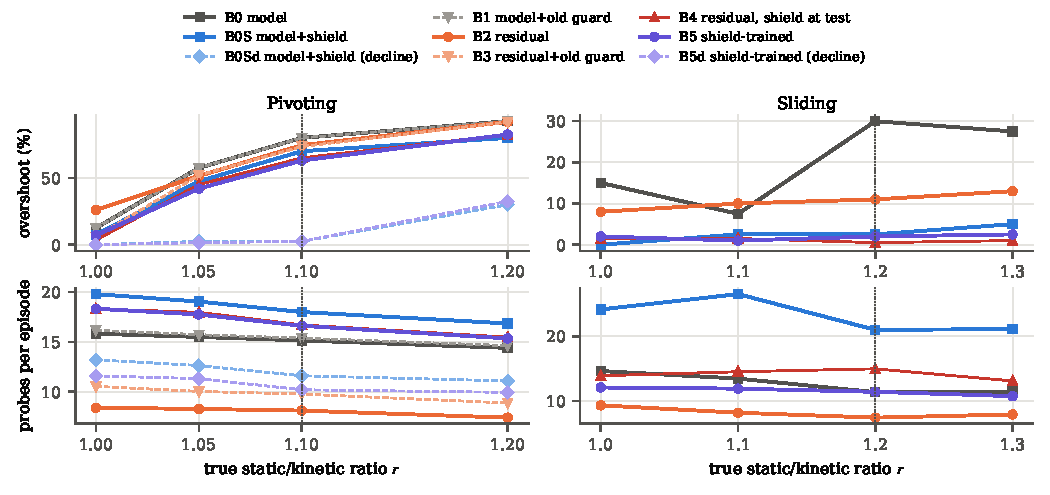
\includegraphics[width=\textwidth]{fig_vs_r.pdf}
\caption{Overshoot rate (top) and probes per episode (bottom) against the true static/kinetic ratio $r$, on the test sets. Dotted vertical line: the shield's assumed $r_{\max}$. In sliding the shield-trained residual (B5) stays near zero overshoot across $r$. In pivoting only the decline fallbacks (B0Sd, B5d) prevent overshoot, by stopping short.}\label{fig:vsr}
\end{figure*}

\subsection{Q3: How much of the task admits a certified action?}
\emph{Pivoting} is limited by Eq.~\eqref{eq:feas}. With $r_{\max}=1.1$, the equation predicts that 20 of the 40 test targets have no certified release from rest. The model controller with the decline fallback (B0Sd) declined at its very first step on exactly these 20 objects, both at $r=1.0$ and at $r=1.1$. A further 14 (at $r=1.0$) and 11 (at $r=1.1$) declined later, after 5--28 steps, once the rod had moved part of the way and the remaining arc could no longer be certified. Overall B0Sd declined on \N{pivot-1.0-B0Sd-declined}, \N{pivot-1.05-B0Sd-declined}, \N{pivot-1.1-B0Sd-declined} and \N{pivot-1.2-B0Sd-declined} of 40 objects. With the defer fallback, 53--61\% of steps were certified. The infeasible region is therefore not a corner case: for realistic friction ratios it covers most of the task.


\emph{Sliding} behaves as Proposition~\ref{prop:slide} predicts. Every shielded episode deferred exactly once, on its first pulse, while $F_{\rm stuck}$ was still unknown. No later pulse was infeasible, at any $r$ (B0S 160 of 160 episodes, B4 and B5 800 of 800 each).

\subsection{Q4: Why do violations and overshoots occur?}\label{sec:q4}
\emph{Attribution.} We replayed every test episode with a certificate violation and classified each violating step (an exploratory analysis, run after the pre-registered tests). For sliding, 10 of the 32 violating steps occurred at $r=1.3>r_{\max}$, where no guarantee applies. One followed a recorded stuck grip that was below the true arrest requirement: the rod had slipped by less than the 2.5\,mm motion threshold. The remaining 21 occurred with every assumption of Proposition~\ref{prop:slide} satisfied. All 21 were on three objects, all heavy ($m=0.178$--$0.192$\,kg). Direct probes on these objects found simulated travel up to 1.8 times the bound for short pulses released close to the stuck grip, where the bound is only a few millimetres. On light objects, travel stayed below the bound. We attribute these to MuJoCo's regularised friction, which lets a heavily loaded contact creep \cite{mujocoissue}; this is a simulator effect and not a sensing error.

For pivoting, violations rise roughly tenfold when the assumption fails: at $r=1.2>r_{\max}$, \N{pivot-1.2-B5-viol} of \N{pivot-1.2-B5-cert} certified B5 steps (\N{pivot-1.2-B5-violpct}\%) violated the certificate, and decline-mode overshoot rose to \N{pivot-1.2-B5d-over}\%. At $r\le r_{\max}$ the violation rate is consistent with the model--simulator gap measured in V6.

\emph{Mismatch.} Fig.~\ref{fig:mismatch} shows what happens when $r_{\max}$ is wrong. In sliding, assuming $r_{\max}=1.0$ when the true $r$ is 1.1 or 1.2 raises B5's overshoot to \N{slide-mis-r1.1_rmax1.0-B5-over} and \N{slide-mis-r1.2_rmax1.0-B5-over}\% and its violation rate to about 1\%. Its probes fall to \N{slide-mis-r1.2_rmax1.0-B5-probes}, the level of the unshielded residual. Assuming $r_{\max}=1.3$ keeps overshoot at \N{slide-mis-r1.2_rmax1.3-B5-over}--\N{slide-mis-r1.1_rmax1.3-B5-over}\% at a cost of \N{slide-mis-r1.2_rmax1.3-B5-probes} probes. The bound trades measurements for overshoot monotonically, and an underestimate degrades the shield gradually rather than abruptly. Pivoting behaves differently. With $r_{\max}=1.0$ every step is certifiable, but the certificates are wrong: \N{pivot-mis-r1.1_rmax1.0-B5-violpct}\% of B5's certified steps violated them at $r=1.1$. Yet B5's overshoot (\N{pivot-mis-r1.1_rmax1.0-B5-over}\%) is \emph{lower} than with $r_{\max}=1.2$ (\N{pivot-mis-r1.1_rmax1.2-B5-over}\%), where about 80\% of steps are deferred and no certificate is violated. A larger $r_{\max}$ hands more steps back to the model, which overshoots. With the defer fallback, a valid certificate on every certified step does not make the episode safe.

\begin{figure}[t]\centering
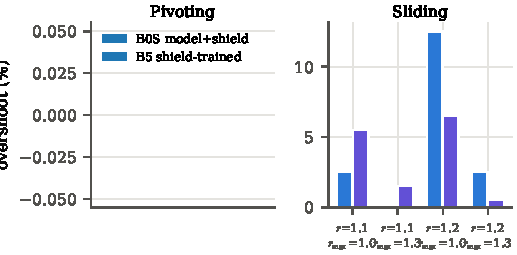
\includegraphics[width=\columnwidth]{fig_mismatch.pdf}
\caption{Overshoot of the shield-trained residual (B5, defer fallback) when the assumed $r_{\max}$ is wrong. Pivoting: $r_{\max}=1.0$, 1.1 (as trained) and 1.2. Sliding: 1.0, 1.2 (as trained) and 1.3. In sliding an underestimate raises overshoot and an overestimate lowers it. In pivoting the order reverses, because a larger $r_{\max}$ defers more steps to the overshooting model controller.}\label{fig:mismatch}
\end{figure}

\emph{Confirmation.} The confirmation sets, 40 fresh objects per task with $r$ drawn from the training range, were each run once after the test analysis had been committed. In sliding, B5 overshot \N{slide-conf-B5-over}\% of episodes against \N{slide-conf-B0-over}\% for B0 (Wilcoxon $p\N{slide-conf-B5-povershoot}$), ended within 5\,mm in \N{slide-conf-B5-within}\% against \N{slide-conf-B0-within}\%, and used \N{slide-conf-B5-probes} probes against \N{slide-conf-B0-probes} (difference not significant). The test-set conclusions replicate.
In pivoting ($r$ drawn from $[1.0,1.1]$), the confirmation set again showed no safety gain from the defer fallback: B5 overshot \N{pivot-conf-B5-over}\% against \N{pivot-conf-B0-over}\% for B0, while using \N{pivot-conf-B5-probes} probes against \N{pivot-conf-B0-probes} (Wilcoxon $p\N{pivot-conf-B5-pprobes}$). The decline fallback again removed overshoot (B0Sd \N{pivot-conf-B0Sd-over}\%) but declined on \N{pivot-conf-B0Sd-declined} of 40 objects and ended within the band on \N{pivot-conf-B0Sd-within}\%. No certified B5 step violated its certificate (\N{pivot-conf-B5-viol} of \N{pivot-conf-B5-cert}).
